% numerical.tex

\cleardoublepage
\chapter{Optimised Trajectory Including Fly-Back}\label{chapter:Flyback}

This chapter presents the maximum payload-to-orbit optimised trajectory of the rocket-scramjet-rocket launch system, including the fly-back of the SPARTAN. 
 Returning the SPARTAN for landing at the initial launch site allows for rapid refurbishment and re-use, and is one of the primary enabling factors in the cost efficient operation of the launch system. 
The fly-back of the SPARTAN requires a full turn-around of the SPARTAN, a glide which covers the necessary ground distance for return, and a deceleration which reduces the speed of the SPARTAN to landing approach velocity, while maintaining suitable high trajectory angle to allow for a controlled approach. 
The return of the SPARTAN to the initial launch site is included in the optimisation process, to maximise the overall efficiency of the launch system. 
This chapter includes a sensitivity analysis, with the same design parameters varied as in the preceding chapter. This sensitivity analysis allows the influence of the fly-back of the SPARTAN on the design sensitivities of the launch system to be assessed.


\section{Combined SPARTAN Ascent-Descent \& Third Stage}
\begin{table}[ht]
	\centering
\begin{tabular}{l c } 
	\hline \textbf{Trajectory Condition}
	& Standard

	\\
	\hline \textbf{Payload to Orbit (kg)}
	& \PayloadToOrbitStandard
	\\
	\textbf{Separation Alt, 1$\rightarrow$2 (km)}
	& \firstsecondSeparationAltStandard
	\\
	\textbf{Separation v, 1$\rightarrow$2 (m/s)}
	& \firstsecondSeparationvStandard
	\\
	\textbf{Separation $\gamma$, 1$\rightarrow$2 (m/s)}
	& \firstsecondSeparationgammaStandard
	\\
	\textbf{Separation Alt, 2$\rightarrow$3 (km)}
	& \secondthirdSeparationAltStandard
	\\
	\textbf{Separation $v$, 2$\rightarrow$3 (m/s)}
	& \secondthirdSeparationvStandard
	\\
	\textbf{Separation $\gamma$, 2$\rightarrow$3 (deg)}
	& \secondthirdSeparationgammaStandard
	\\
	\textbf{Separation $q$, 2$\rightarrow$3(kPa)}
	& \secondthirdSeparationqStandard
	\\
	\textbf{2$^{nd}$ Stage L/D, 2$\rightarrow$3}
	& \secondthirdSeparationLDStandard
	\\
	\textbf{2$^{nd}$ Stage Flight Time (s)}
	& \secondFlightTimeStandard
	\\
	\textbf{2$^{nd}$ Stage Return Fuel (kg)}
	& \returnFuelStandard
	\\
	\textbf{3$^{rd}$ Stage $t$, $q >$ 5kpa (s)}
	& \thirdqOverFiveStandard
	\\
	\textbf{3$^{rd}$ Stage max $\alpha$ (deg)}
	& \thirdmaxAoAStandard
	\\
	\textbf{3$^{rd}$ Stage final v (m/s)}
	& \thirdcircvStandard
	\\
	\textbf{3$^{rd}$ Stage final m (kg)}
	& \thirdcircmStandard
	\\
	\hline 
\end{tabular} 
\end{table}

The trajectory of the rocket-scramjet-rocket launch system has been optimised in LODESTAR, including the return of the SPARTAN to its initial launch site. The optimised trajectory is shown in Figure \ref{fig:GroundTrackStandard}. 
The rocket-scramjet-rocket launch system is shown to be able to launch a small satellite 
while flying-back the SPARTAN to the initial launch site location, and approaching the landing site at appropriately low altitude and velocity to allow for landing on a traditional runway. 
The optimised trajectory attains a payload mass to SSO of \PayloadToOrbitStandard kg. 
This indicates that the launch system utilising the SPARTAN is capable of successfully completing a small satellite launch mission which allows for rapid reusability of the SPARTAN. 
\begin{figure}[ht!]
	\centering
	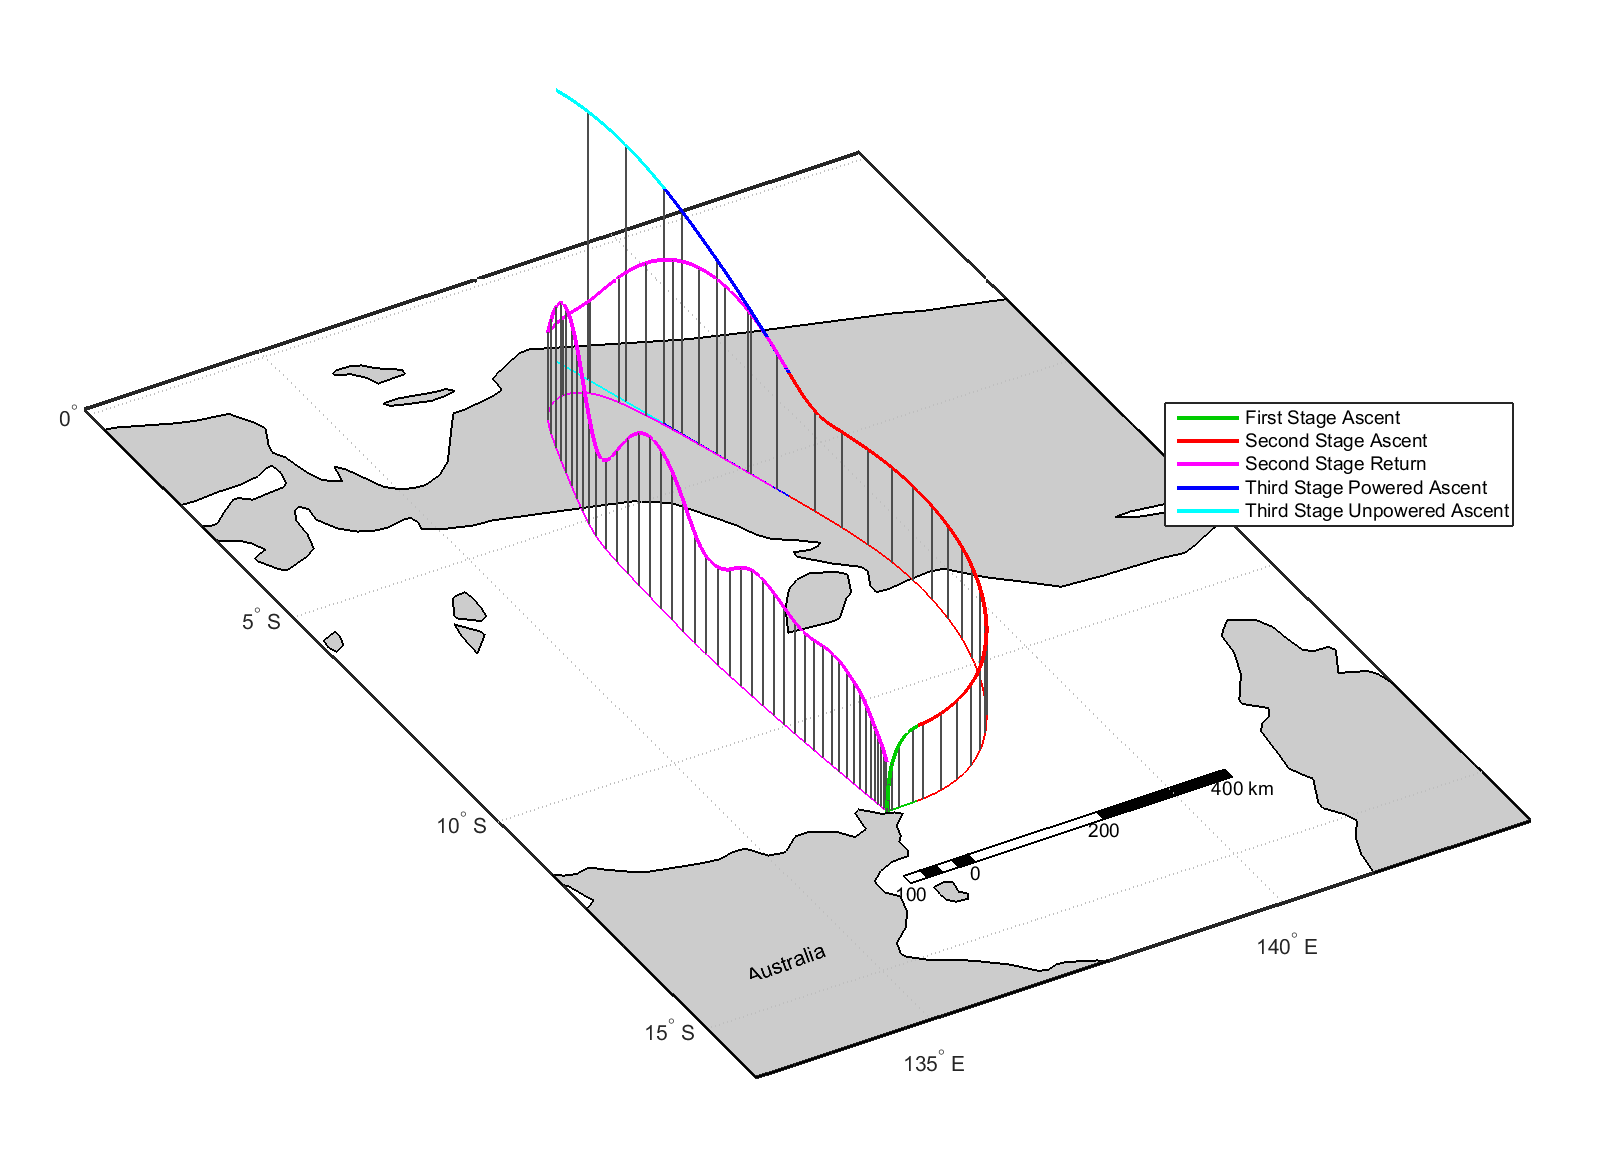
\includegraphics[width=1\linewidth]{../LODESTAR_FINAL/Results/mode11/GroundTrackStandard}
	\caption{}
	\label{fig:GroundTrackStandard}
\end{figure}
The maximum payload-to-orbit is reduced by XX\% compared to the optimised trajectory result without fly-back. The benefits of flying back the SPARTAN to its initial launch site, compared to the alternative of transporting the SPARTAN back to the launch site from a remote landing, are likely to far outweigh this associated reduction in payload. 


\section{Ascent Trajectory}

 The initial launch for a maximum payload-to-orbit trajectory with SPARTAN fly-back is to the east.
 The first stage trajectory is very similar to that of the first stage launching the SPARTAN with no return flight, detailed in Section \ref{sec:optimisednoreturn}, and is shown in Appendix \ref{sec:appendix_firststage}. 
 After the easterly launch, and first stage pitchover, the SPARTAN is released in an easterly direction, and performs a banking manoeuvre throughout its acceleration so that the heading angle is pointed appropriately close to north-northwest at the release of the third stage rocket. 
\begin{figure}[ht!]
\centering
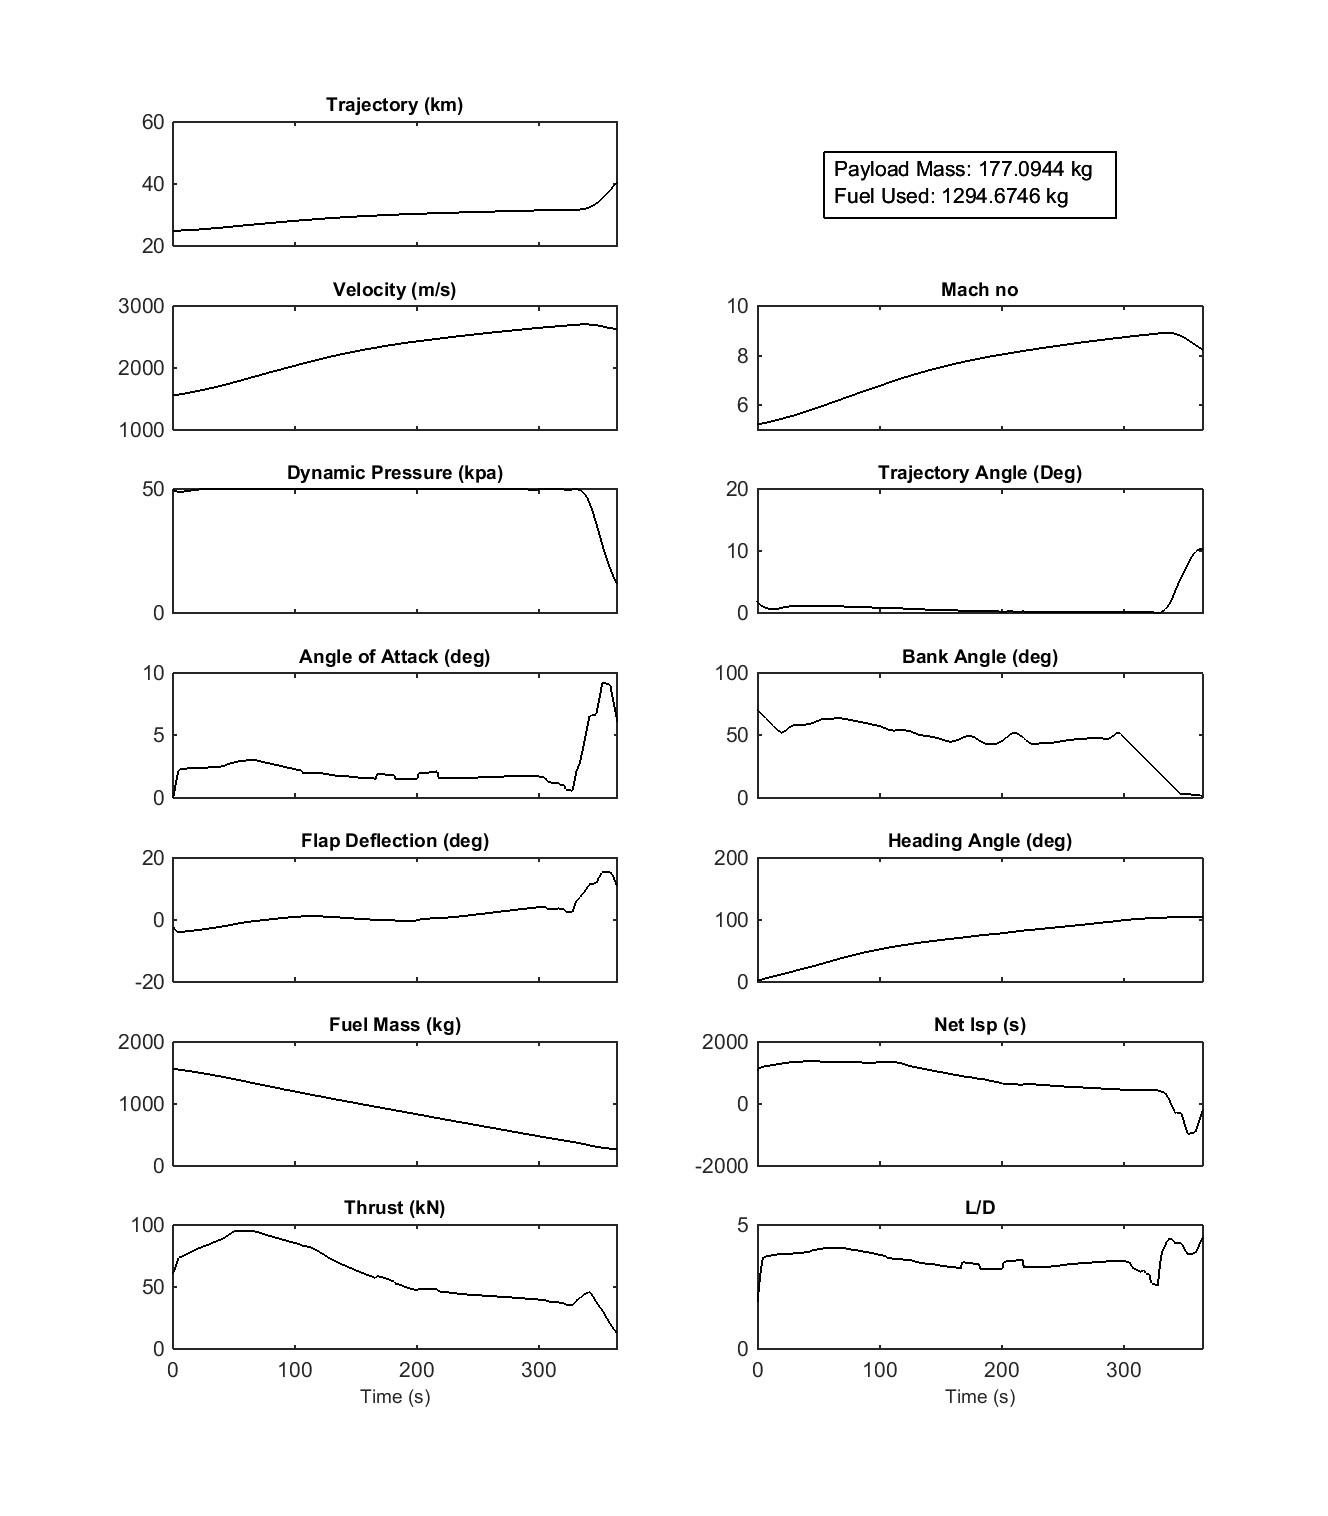
\includegraphics[width=1\linewidth]{../LODESTAR_FINAL/Results/mode11/SecondStageStandard}
\caption{}
\label{fig:SecondStageStandard}
\end{figure}
\begin{figure}[ht!]
\centering
\includegraphics[width=0.9\linewidth]{../LODESTAR_FINAL/Results/mode11/NetIspStandard}
\caption{}
\label{fig:NetIspStandard}
\end{figure}
During the ascent, the bank angle of the SPARTAN is significantly large and the angle of attack of the SPARTAN is significantly higher than during the maximum payload-to-orbit trajectory with no fly-back, detailed in Section XX.
As a consequence, the net specific impulse of the SPARTAN is decreased during its acceleration, which can be observed in Figure \ref{fig:NetIspStandard}. This higher angle of attack results in no altitude raising manoeuvre in the middle of the acceleration trajectory of the SPARTAN. The SPARTAN no longer flies within the homogeneous region of the specific impulse of the C-REST engines, instead the flight conditions are close to a region where an increase in angle of attack causes a sharp decrease in specific impulse. 
This indicates that at Mach 7 and 8 the angle of attack, and consequently, the allowable bank angle, of the SPARTAN may be being limited by the performance of the C-REST engines. 

 The bank angle is initially 75.4 $^\circ$ at the first stage-SPARTAN separation, which aids the SPARTAN in decreasing its altitude to close to maximum dynamic pressure at 64.9s. The bank angle decreases as the SPARTAN reaches its maximum dynamic pressure, then adjusts and stays between 52.4$^\circ$ - 58.7$^\circ$ for the duration of the acceleration, until a pull-up is performed at 341.2s. During the pull-up, the bank angle is steadily reduced at its maximum change rate, until the release of the third stage rocket at 0$^\circ$ bank angle. 

A total fuel mass of 1307.5kg is used during the SPARTAN's acceleration. This reduction in fuel mass used, along with the reduction in net specific impulse due to the higher angle of attack values, reduces the velocity at SPARTAN-third stage separation by XXm/s compared to the maximum payload-to-orbit case with no SPARTAN fly-back. The SPARTAN pulls up to \secondthirdSeparationAltStandard km altitude and \secondthirdSeparationgammaStandard $^\circ$ before SPARTAN-third stage separation, a difference of only XXkm and XX$^\circ$ compared to the maximum payload-to-orbit trajectory without fly-back. 



\begin{figure}[ht!]
\centering
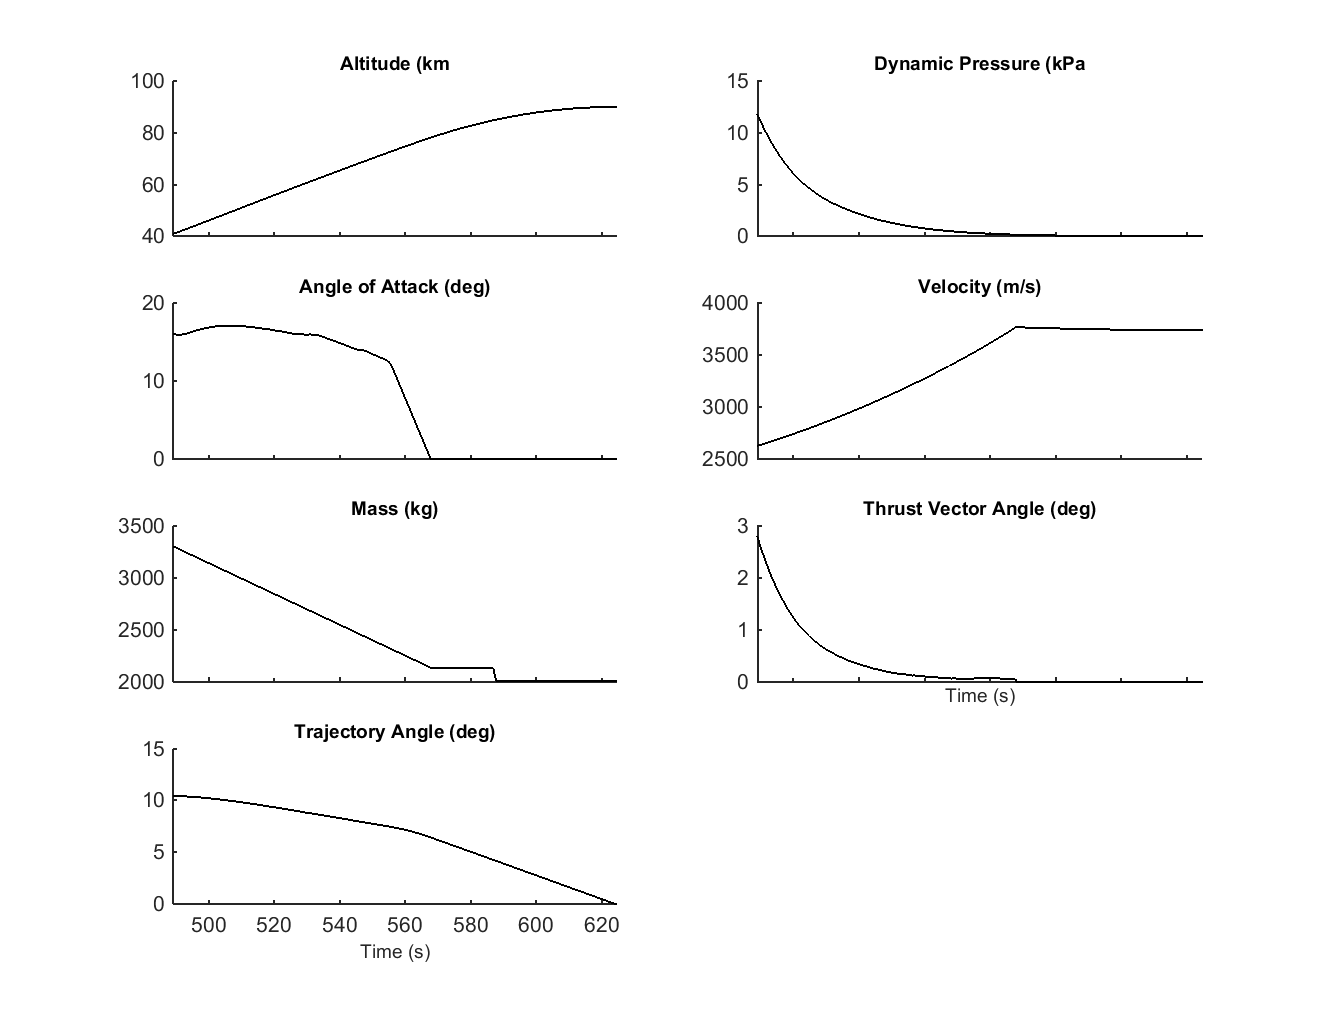
\includegraphics[width=1\linewidth]{../LODESTAR_FINAL/Results/mode11/ThirdStageStandard}
\caption{}
\label{fig:ThirdStageStandard}
\end{figure}


\section{Fly-Back Trajectory}

\begin{figure}[ht!]
	\centering
	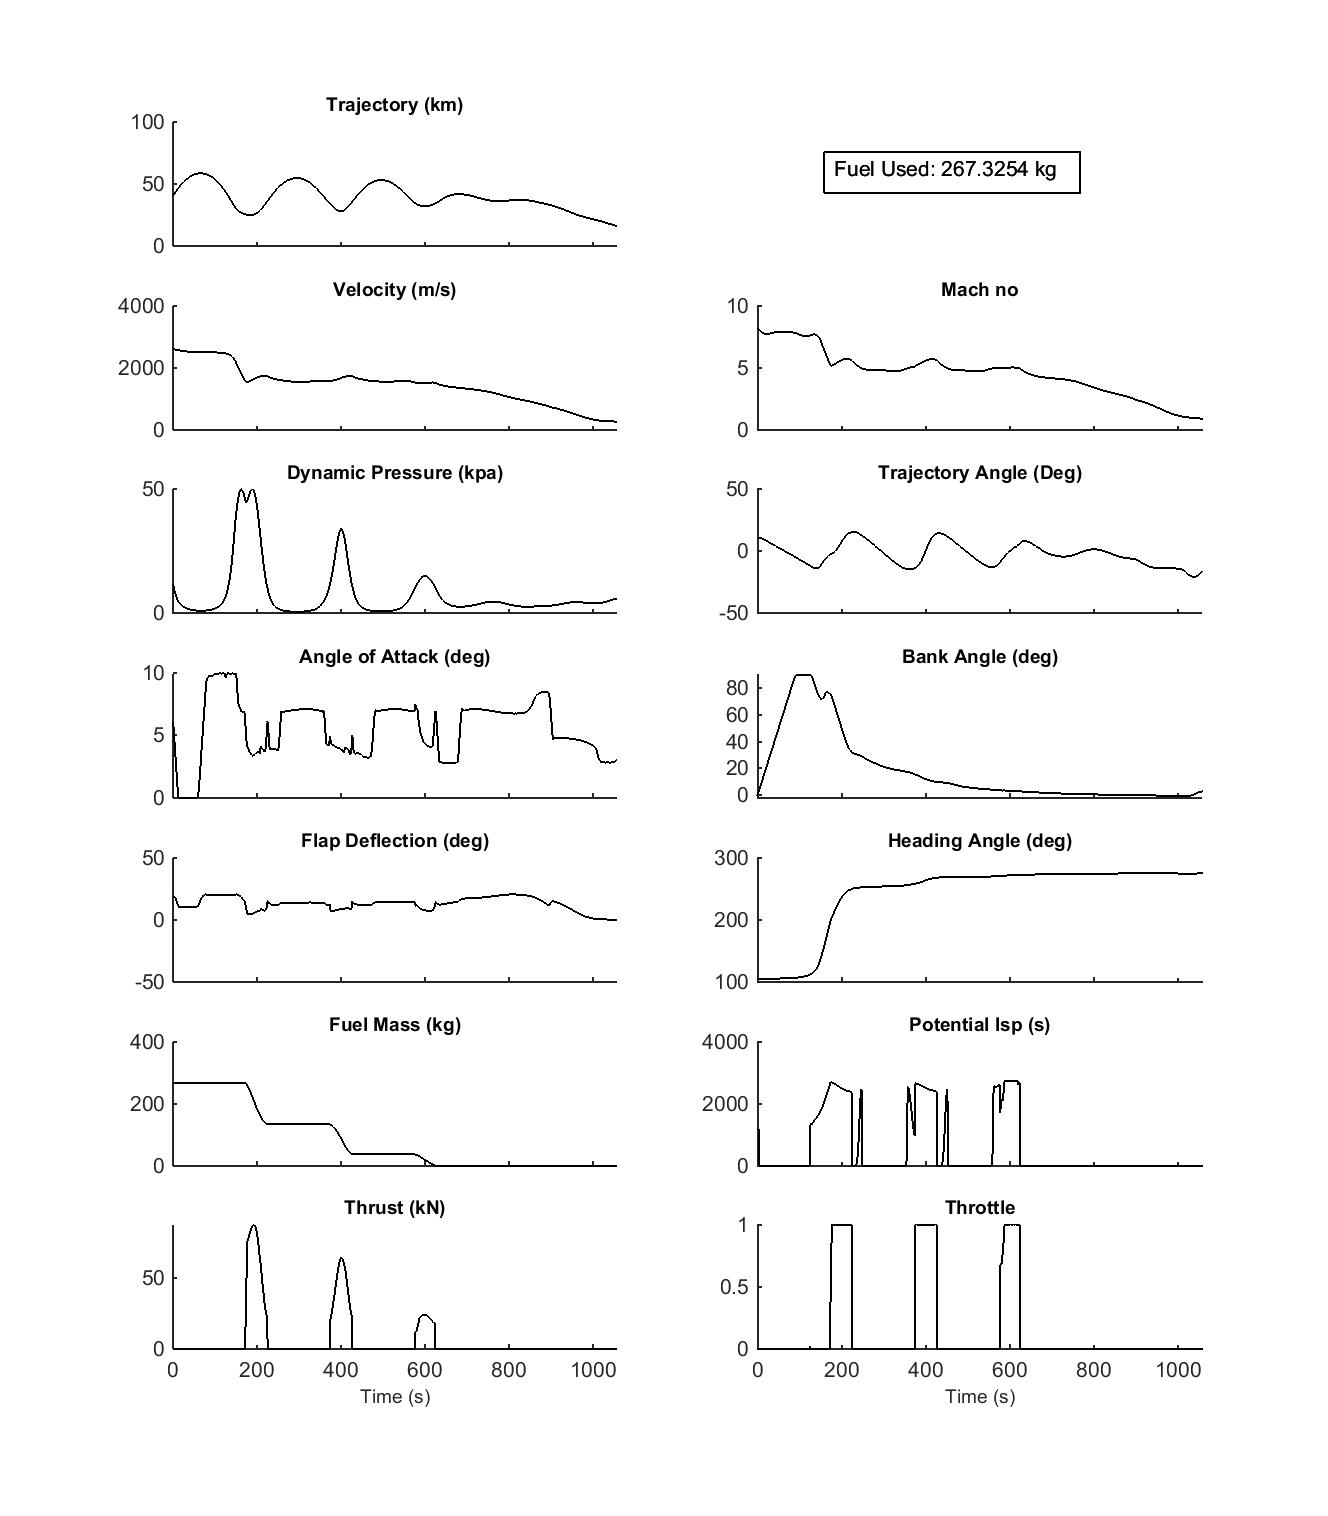
\includegraphics[width=1\linewidth]{../LODESTAR_FINAL/Results/mode11/ReturnStandard}
	\caption{}
	\label{fig:ReturnStandard}
\end{figure}

The optimised fly-back trajectory is shown in Figure \ref{fig:ReturnStandard}.
The SPARTAN is shown to be capable of fly-back, using 254.5kg of fuel, 16.3\% of the total fuel.
The optimised trajectory has four distinct parts; 1. initial turn, 2. boost phase, 3. hop-glide, and 4. approach. 

\subsubsection{ Initial Turn}
The SPARTAN separates from the third stage rocket at a bank angle of 0$^\circ$, and then increases the bank angle at its maximum change rate until 98.5s and 89.5$^\circ$ bank angle. At this point, the altitude of the SPARTAN is decreasing, and the SPARTAN rapidly becomes close to hitting the dynamic pressure of 50kPa. To avoid exceeding this limit, the bank angle is reduced to 67.5$^\circ$ at 164.3s, allowing the vehicle to generate sufficient lift to slow its descent. 

\subsubsection{ Boost Phase}
Soon after the bank angle has reduced to 67.5$^\circ$, the scramjet engines are ignited. The C-REST engines are powered-on at a point of high potential specific impulse, at a low Mach number, and burn for 46.5s. The altitude of the SPARTAN is raised during the initial burn, ensuring that the Mach number is kept low for maximum efficiency. The maximum altitude during the burn is limited by the lower dynamic pressure limit of the C-REST engines of 20kPa. At 227.9s, the initial burn ends, the angle of attack of the SPARTAN is decreased to 1.27$^\circ$, and the altitude decreases. As soon as the dynamic pressure is high enough for C-REST engine operation at 259.5s, the scramjet engines are once again ignited. During the second burn, the bank angle of the vehicle is reduced to produce increased lift, so as to increase the altitude of the SPARTAN, while also maximising the specific impulse of the scramjet engines by keeping the angle of attack low. The low angle of attack values decrease the temperature and raise the Mach number at the inlet of the C-REST engines. While these effects partially offset each other\cite{Preller2017}, the temperature increase is more significant, and decreasing the angle of attack has the net effect of increasing the specific impulse of the C-REST engines. This increase in specific impulse is balanced by a decrease in the L/D of the SPARTAN at angle of attack values lower than 4$^\circ$, as illustrated in Figure \ref{fig:LD}. However, the specific impulse has a more significant impact than the L/D during this phase, resulting in the optimised angle of attack being kept low. The angle of attack is increased gradually during the burn, increasing the L/D of the vehicle and initiating a large 'skip'. 
This skip raises the altitude of the SPARTAN to 49.0km, before it decreases once again. 
The third and last burn is initiated as the altitude of the SPARTAN is still decreasing, at 458.1s and lasts until 513.1s, when the remaining fuel has been depleted. 



\subsubsection{ Skip-Glide}

 The skips which the SPARTAN exhibits during its return flight are aided by the angle of attack of the SPARTAN, and are consistent with research which has shown that a periodic skipping trajectory increases the downrange distance achievable by hypersonic vehicles both during powered and unpowered flight\cite{Eggers1957,Kanda2007}. 
During the unpowered trajectory after the burn phase, the angle of attack is initially controlled so that the L/D of the SPARTAN is close to the maximum, and the lift of the SPARTAN is high. This high angle of attack is sustained until 694.2s, when the Mach number has fallen below 4, so that the SPARTAN is in a region of low L/D, and the fifth skip has begun. At this point, the angle of attack is reduced significantly, to 2.6$^\circ$, reducing the size of the fifth skip. At 803.0s, the angle of attack is again raised to 4.9$^\circ$, initiating the sixth and last skip. After this increase, the angle of attack is adjusted, so that as the SPARTAN completes the final skip, a gradual, controlled descent is initiated. 




\subsubsection{ Approach}
After the skip phase, as the vehicle is approaching Mach 1, the angle of attack is reduced gradually to bring the SPARTAN down to 1km altitude, in a controlled manner. At 1130.0s, the bank angle is increased, in order to perform a final adjustment of the heading angle, to bring the SPARTAN to the desired end location. 
The SPARTAN reaches 1km altitude at -32.5$^\circ$ trajectory angle and 124.9m/s velocity, and it is assumed that the SPARTAN is able to perform a landing manoeuvre after this point. 








\subsection{Design Sensitivity Analysis}

During the preliminary stages of launch vehicle design, it is important to characterise the effects of changes in the design of a vehicle.  
Quantifying the effects of variations within the vehicle design allows the vehicle performance to be improved. 
However, the complete assessment of the effects of vehicle design variations requires every critical feature of the design to be modified, and the new vehicle design to be investigated. This method of investigation is prohibitively time consuming and computationally expensive for a complex launch system. Consequently, it is important to first understand the effects of the key performance parameters of the vehicle, so that when the design of the launch system is to be iterated, the design of each vehicle and subsystem may be tailored towards improving the overall performance.
 The this end, a sensitivity study is performed to investigate the variations in the optimal trajectory when key performance parameters of the vehicle are modified.

The performance parameters modified are:

\begin{itemize}
	\item Maximum dynamic pressure.
	\item Specific Impulse of the C-REST engines. 
	\item SPARTAN aerodynamic drag.
	\item SPARTAN mass.
	\item SPARTAN fuel mass.
	\item Third stage mass.
	\item Third stage thrust. 
	\item SPARTAN viscous drag. 
	
\end{itemize}



 These parameters are varied and the new optimal fly-back trajectories are calculated using LODESTAR. These optimised trajectories are detailed in the following sections.
 
The consistency of the trajectory shape indicates that the optimal solution is robust with variation in the aerodynamic parameters and specific impulse of the SPARTAN. The optimised trajectories show clear trends with variation in vehicle parameters.






\section{dynamic pressure}

The maximum dynamic pressure  of the SPARTAN has a significantly increased effect on the maximum payload-to-orbit optimised trajectory which includes the SPARTAN flying-back to the launch site. This is primarily due to the increased maximum dynamic pressure improving the manoeuvring capabilities of the SPARTAN and increasing the acceleration rate during ascent, which leads to a smaller flight time, and less ground coverage. 

\begin{table}[ht]
\centering
\begin{tabular}{l c c c c c c} 
	\hline \textbf{Trajectory Condition}
	& q40
	& q45
	& q100
	& q55
	& q60
	& /\%
	\\
	\hline \textbf{Payload to Orbit (kg)}
	& \PayloadToOrbitqForty
	& \PayloadToOrbitqFortyFive
	& \PayloadToOrbitqStandard
	& \PayloadToOrbitqFiftyFive
	& \PayloadToOrbitqSixty
	&0.4
	\\
	\textbf{Separation Alt, 1$\rightarrow$2 (km)}
	& \firstsecondSeparationAltqForty
	& \firstsecondSeparationAltqFortyFive
	& \firstsecondSeparationAltqStandard
	& \firstsecondSeparationAltqFiftyFive
	& \firstsecondSeparationAltqSixty
	& -
	\\
	\textbf{Separation v, 1$\rightarrow$2 (m/s)}
	& \firstsecondSeparationvqForty
	& \firstsecondSeparationvqFortyFive
	& \firstsecondSeparationvqStandard
	& \firstsecondSeparationvqFiftyFive
	& \firstsecondSeparationvqSixty
	& -
	\\
	\textbf{Separation $\gamma$, 1$\rightarrow$2 (m/s)}
	& \firstsecondSeparationgammaqForty
	& \firstsecondSeparationgammaqFortyFive
	& \firstsecondSeparationgammaqStandard
	& \firstsecondSeparationgammaqFiftyFive
	& \firstsecondSeparationgammaqSixty
	& -
	\\
	\textbf{Separation Alt, 2$\rightarrow$3 (km)}
	& \secondthirdSeparationAltqForty
	& \secondthirdSeparationAltqFortyFive
	& \secondthirdSeparationAltqStandard
	& \secondthirdSeparationAltqFiftyFive
	& \secondthirdSeparationAltqSixty
	& -
	\\
	\textbf{Separation $v$, 2$\rightarrow$3 (m/s)}
	& \secondthirdSeparationvqForty
	& \secondthirdSeparationvqFortyFive
	& \secondthirdSeparationvqStandard
	& \secondthirdSeparationvqFiftyFive
	& \secondthirdSeparationvqSixty
	&2.02
	\\
	\textbf{Separation $\gamma$, 2$\rightarrow$3 (deg)}
	& \secondthirdSeparationgammaqForty
	& \secondthirdSeparationgammaqFortyFive
	& \secondthirdSeparationgammaqStandard
	& \secondthirdSeparationgammaqFiftyFive
	& \secondthirdSeparationgammaqSixty
	& -
	\\
	\textbf{Separation $q$, 2$\rightarrow$3(kPa)}
	& \secondthirdSeparationqqForty
	& \secondthirdSeparationqqFortyFive
	& \secondthirdSeparationqqStandard
	& \secondthirdSeparationqqFiftyFive
	& \secondthirdSeparationqqSixty
	&0.04
	\\
	\textbf{2$^{nd}$ Stage L/D, 2$\rightarrow$3}
	& \secondthirdSeparationLDqForty
	& \secondthirdSeparationLDqFortyFive
	& \secondthirdSeparationLDqStandard
	& \secondthirdSeparationLDqFiftyFive
	& \secondthirdSeparationLDqSixty
	&0.02
	\\
	\textbf{2$^{nd}$ Stage Flight Time (s)}
	& \secondFlightTimeqForty
	& \secondFlightTimeqFortyFive
	& \secondFlightTimeqStandard
	& \secondFlightTimeqFiftyFive
	& \secondFlightTimeqSixty
	&-2.49
	\\
	\textbf{2$^{nd}$ Stage Return Fuel (kg)}
	& \returnFuelqForty
	& \returnFuelqFortyFive
	& \returnFuelqStandard
	& \returnFuelqFiftyFive
	& \returnFuelqSixty
	&-1.54
	\\
	\textbf{3$^{rd}$ Stage $t$, $q >$ 5kpa (s)}
	& \thirdqOverFiveqForty
	& \thirdqOverFiveqFortyFive
	& \thirdqOverFiveqStandard
	& \thirdqOverFiveqFiftyFive
	& \thirdqOverFiveqSixty
	& -
	\\
	\textbf{3$^{rd}$ Stage max $\alpha$ (deg)}
	& \thirdmaxAoAqForty
	& \thirdmaxAoAqFortyFive
	& \thirdmaxAoAqStandard
	& \thirdmaxAoAqFiftyFive
	& \thirdmaxAoAqSixty
	& 0
	\\
	\textbf{3$^{rd}$ Stage final v (m/s)}
	& \thirdcircvqForty
	& \thirdcircvqFortyFive
	& \thirdcircvqStandard
	& \thirdcircvqFiftyFive
	& \thirdcircvqSixty
	& -
	\\
	\textbf{3$^{rd}$ Stage final m (kg)}
	& \thirdcircmqForty
	& \thirdcircmqFortyFive
	& \thirdcircmqStandard
	& \thirdcircmqFiftyFive
	& \thirdcircmqSixty
	& -
	\\
	\hline 
\end{tabular} 
\end{table}


\section{Isp}


Increasing the specific impulse causes the fuel necessary for fly-back to decrease by -XXkg (-XX\%), while decreasing the specific impulse causes the fuel necessary to rise by +XXkg (+XX\%). The start of scramjet burn is consistent across different specific impulse test cases. Due to the increase in thrust, the SPARTAN accelerates more rapidly for the higher specific impulse case. As a consequence, the initial 'skip' is performed sooner.

\begin{table}[ht]
	\centering
\begin{tabular}{l c c c c c c} 
	\hline \textbf{Trajectory Condition}
	&Isp90
	&Isp95
	&Isp100
	&Isp105
	&Isp110
	& /\%
	\\
	\hline \textbf{Payload to Orbit (kg)}
	& \PayloadToOrbitIspNinety
	& \PayloadToOrbitIspNinetyFive
	& \PayloadToOrbitIspStandard
	& \PayloadToOrbitIspOneHundredFive
	& \PayloadToOrbitIspOneHundredTen
	&1.7
	\\
	\textbf{Separation Alt, 1$\rightarrow$2 (km)}
	& \firstsecondSeparationAltIspNinety
	& \firstsecondSeparationAltIspNinetyFive
	& \firstsecondSeparationAltIspStandard
	& \firstsecondSeparationAltIspOneHundredFive
	& \firstsecondSeparationAltIspOneHundredTen
	& -
	\\
	\textbf{Separation v, 1$\rightarrow$2 (m/s)}
	& \firstsecondSeparationvIspNinety
	& \firstsecondSeparationvIspNinetyFive
	& \firstsecondSeparationvIspStandard
	& \firstsecondSeparationvIspOneHundredFive
	& \firstsecondSeparationvIspOneHundredTen
	& -
	\\
	\textbf{Separation $\gamma$, 1$\rightarrow$2 (m/s)}
	& \firstsecondSeparationgammaIspNinety
	& \firstsecondSeparationgammaIspNinetyFive
	& \firstsecondSeparationgammaIspStandard
	& \firstsecondSeparationgammaIspOneHundredFive
	& \firstsecondSeparationgammaIspOneHundredTen
	& -
	\\
	\textbf{Separation Alt, 2$\rightarrow$3 (km)}
	& \secondthirdSeparationAltIspNinety
	& \secondthirdSeparationAltIspNinetyFive
	& \secondthirdSeparationAltIspStandard
	& \secondthirdSeparationAltIspOneHundredFive
	& \secondthirdSeparationAltIspOneHundredTen
	& -
	\\
	\textbf{Separation $v$, 2$\rightarrow$3 (m/s)}
	& \secondthirdSeparationvIspNinety
	& \secondthirdSeparationvIspNinetyFive
	& \secondthirdSeparationvIspStandard
	& \secondthirdSeparationvIspOneHundredFive
	& \secondthirdSeparationvIspOneHundredTen
	&11.13
	\\
	\textbf{Separation $\gamma$, 2$\rightarrow$3 (deg)}
	& \secondthirdSeparationgammaIspNinety
	& \secondthirdSeparationgammaIspNinetyFive
	& \secondthirdSeparationgammaIspStandard
	& \secondthirdSeparationgammaIspOneHundredFive
	& \secondthirdSeparationgammaIspOneHundredTen
	&-0.09
	\\
	\textbf{Separation $q$, 2$\rightarrow$3(kPa)}
	& \secondthirdSeparationqIspNinety
	& \secondthirdSeparationqIspNinetyFive
	& \secondthirdSeparationqIspStandard
	& \secondthirdSeparationqIspOneHundredFive
	& \secondthirdSeparationqIspOneHundredTen
	&0.07
	\\
	\textbf{2$^{nd}$ Stage L/D, 2$\rightarrow$3}
	& \secondthirdSeparationLDIspNinety
	& \secondthirdSeparationLDIspNinetyFive
	& \secondthirdSeparationLDIspStandard
	& \secondthirdSeparationLDIspOneHundredFive
	& \secondthirdSeparationLDIspOneHundredTen
	& -
	\\
	\textbf{2$^{nd}$ Stage Flight Time (s)}
	& \secondFlightTimeIspNinety
	& \secondFlightTimeIspNinetyFive
	& \secondFlightTimeIspStandard
	& \secondFlightTimeIspOneHundredFive
	& \secondFlightTimeIspOneHundredTen
	& -
	\\
	\textbf{2$^{nd}$ Stage Return Fuel (kg)}
	& \returnFuelIspNinety
	& \returnFuelIspNinetyFive
	& \returnFuelIspStandard
	& \returnFuelIspOneHundredFive
	& \returnFuelIspOneHundredTen
	& -
	\\
	\textbf{3$^{rd}$ Stage $t$, $q >$ 5kpa (s)}
	& \thirdqOverFiveIspNinety
	& \thirdqOverFiveIspNinetyFive
	& \thirdqOverFiveIspStandard
	& \thirdqOverFiveIspOneHundredFive
	& \thirdqOverFiveIspOneHundredTen
	& -
	\\
	\textbf{3$^{rd}$ Stage max $\alpha$ (deg)}
	& \thirdmaxAoAIspNinety
	& \thirdmaxAoAIspNinetyFive
	& \thirdmaxAoAIspStandard
	& \thirdmaxAoAIspOneHundredFive
	& \thirdmaxAoAIspOneHundredTen
	& -
	\\
	\textbf{3$^{rd}$ Stage final v (m/s)}
	& \thirdcircvIspNinety
	& \thirdcircvIspNinetyFive
	& \thirdcircvIspStandard
	& \thirdcircvIspOneHundredFive
	& \thirdcircvIspOneHundredTen
	&15.17
	\\
	\textbf{3$^{rd}$ Stage final m (kg)}
	& \thirdcircmIspNinety
	& \thirdcircmIspNinetyFive
	& \thirdcircmIspStandard
	& \thirdcircmIspOneHundredFive
	& \thirdcircmIspOneHundredTen
	& -
	\\
	\hline 
\end{tabular} 
	
\end{table}

\section{Cd}

Increasing the drag coefficient causes the fuel necessary for fly-back to increase by +XXkg (+XX\%). Conversely, decreasing the drag coefficient by 10\% causes the fuel necessary for  fly-back to decrease by -XXkg (-XX\%). 
When the drag is increased (ie. L/D is decreased), the scramjet engine burn phase begins earlier, and continues for longer. 
The greater burn time allows the maximum altitude attained during the initial 'skip' to be higher. 
This additional altitude is necessary as the greater drag causes the velocity, and consequentially altitude, of the SPARTAN to decrease more rapidly.

-above currently not correct (potentially, awaiting new results)


-the effect of Cd is reduced compared to the no fly-back case

-some of the negative effects of Cd are offset by the tighter trajectory being flown, and the lower ground distance covered


\begin{table}[ht]
	\centering
	\begin{tabular}{l c c c c c c} 
		\hline \textbf{Trajectory Condition}
		&Cd90
		&Cd95
		&Cd100
		&Cd105
		&Cd110
		& /\%
		\\
		\hline \textbf{Payload to Orbit (kg)}
		& \PayloadToOrbitCdNinety
		& \PayloadToOrbitCdNinetyFive
		& \PayloadToOrbitCdStandard
		& \PayloadToOrbitCdOneHundredFive
		& \PayloadToOrbitCdOneHundredTen
		&-1.5
		\\
		\textbf{Separation Alt, 1$\rightarrow$2 (km)}
		& \firstsecondSeparationAltCdNinety
		& \firstsecondSeparationAltCdNinetyFive
		& \firstsecondSeparationAltCdStandard
		& \firstsecondSeparationAltCdOneHundredFive
		& \firstsecondSeparationAltCdOneHundredTen
		& -
		\\
		\textbf{Separation v, 1$\rightarrow$2 (m/s)}
		& \firstsecondSeparationvCdNinety
		& \firstsecondSeparationvCdNinetyFive
		& \firstsecondSeparationvCdStandard
		& \firstsecondSeparationvCdOneHundredFive
		& \firstsecondSeparationvCdOneHundredTen
		&-3.66
		\\
		\textbf{Separation $\gamma$, 1$\rightarrow$2 (m/s)}
		& \firstsecondSeparationgammaCdNinety
		& \firstsecondSeparationgammaCdNinetyFive
		& \firstsecondSeparationgammaCdStandard
		& \firstsecondSeparationgammaCdOneHundredFive
		& \firstsecondSeparationgammaCdOneHundredTen
		& -
		\\
		\textbf{Separation Alt, 2$\rightarrow$3 (km)}
		& \secondthirdSeparationAltCdNinety
		& \secondthirdSeparationAltCdNinetyFive
		& \secondthirdSeparationAltCdStandard
		& \secondthirdSeparationAltCdOneHundredFive
		& \secondthirdSeparationAltCdOneHundredTen
		&-0.07
		\\
		\textbf{Separation $v$, 2$\rightarrow$3 (m/s)}
		& \secondthirdSeparationvCdNinety
		& \secondthirdSeparationvCdNinetyFive
		& \secondthirdSeparationvCdStandard
		& \secondthirdSeparationvCdOneHundredFive
		& \secondthirdSeparationvCdOneHundredTen
		&-9.27
		\\
		\textbf{Separation $\gamma$, 2$\rightarrow$3 (deg)}
		& \secondthirdSeparationgammaCdNinety
		& \secondthirdSeparationgammaCdNinetyFive
		& \secondthirdSeparationgammaCdStandard
		& \secondthirdSeparationgammaCdOneHundredFive
		& \secondthirdSeparationgammaCdOneHundredTen
		&0.04
		\\
		\textbf{Separation $q$, 2$\rightarrow$3(kPa)}
		& \secondthirdSeparationqCdNinety
		& \secondthirdSeparationqCdNinetyFive
		& \secondthirdSeparationqCdStandard
		& \secondthirdSeparationqCdOneHundredFive
		& \secondthirdSeparationqCdOneHundredTen
		& -
		\\
		\textbf{2$^{nd}$ Stage L/D, 2$\rightarrow$3}
		& \secondthirdSeparationLDCdNinety
		& \secondthirdSeparationLDCdNinetyFive
		& \secondthirdSeparationLDCdStandard
		& \secondthirdSeparationLDCdOneHundredFive
		& \secondthirdSeparationLDCdOneHundredTen
		&-0.05
		\\
		\textbf{2$^{nd}$ Stage Flight Time (s)}
		& \secondFlightTimeCdNinety
		& \secondFlightTimeCdNinetyFive
		& \secondFlightTimeCdStandard
		& \secondFlightTimeCdOneHundredFive
		& \secondFlightTimeCdOneHundredTen
		& -
		\\
		\textbf{2$^{nd}$ Stage Return Fuel (kg)}
		& \returnFuelCdNinety
		& \returnFuelCdNinetyFive
		& \returnFuelCdStandard
		& \returnFuelCdOneHundredFive
		& \returnFuelCdOneHundredTen
		& -
		\\
		\textbf{3$^{rd}$ Stage $t$, $q >$ 5kpa (s)}
		& \thirdqOverFiveCdNinety
		& \thirdqOverFiveCdNinetyFive
		& \thirdqOverFiveCdStandard
		& \thirdqOverFiveCdOneHundredFive
		& \thirdqOverFiveCdOneHundredTen
		& -
		\\
		\textbf{3$^{rd}$ Stage max $\alpha$ (deg)}
		& \thirdmaxAoACdNinety
		& \thirdmaxAoACdNinetyFive
		& \thirdmaxAoACdStandard
		& \thirdmaxAoACdOneHundredFive
		& \thirdmaxAoACdOneHundredTen
		& -
		\\
		\textbf{3$^{rd}$ Stage final v (m/s)}
		& \thirdcircvCdNinety
		& \thirdcircvCdNinetyFive
		& \thirdcircvCdStandard
		& \thirdcircvCdOneHundredFive
		& \thirdcircvCdOneHundredTen
		& -
		\\
		\textbf{3$^{rd}$ Stage final m (kg)}
		& \thirdcircmCdNinety
		& \thirdcircmCdNinetyFive
		& \thirdcircmCdStandard
		& \thirdcircmCdOneHundredFive
		& \thirdcircmCdOneHundredTen
		& -
		\\
		\hline 
	\end{tabular} 
\end{table}


\section{m SPARTAN}


\begin{table}[ht]
\centering
\begin{tabular}{l c c c c c c} 
	\hline \textbf{Trajectory Condition}
	&m295
	&m297.5
	&m2100
	&m2102.5
	&m2105
	& /\%
	\\
	\hline \textbf{Payload to Orbit (kg)}
	& \PayloadToOrbitmSPARTANNinetyFive
	& \PayloadToOrbitmSPARTANNinetySevenFive
	& \PayloadToOrbitmSPARTANStandard
	& \PayloadToOrbitmSPARTANOneHundredTwoFive
	& \PayloadToOrbitmSPARTANOneHundredFive
	&-1.2
	\\
	\textbf{Separation Alt, 1$\rightarrow$2 (km)}
	& \firstsecondSeparationAltmSPARTANNinetyFive
	& \firstsecondSeparationAltmSPARTANNinetySevenFive
	& \firstsecondSeparationAltmSPARTANStandard
	& \firstsecondSeparationAltmSPARTANOneHundredTwoFive
	& \firstsecondSeparationAltmSPARTANOneHundredFive
	& -
	\\
	\textbf{Separation v, 1$\rightarrow$2 (m/s)}
	& \firstsecondSeparationvmSPARTANNinetyFive
	& \firstsecondSeparationvmSPARTANNinetySevenFive
	& \firstsecondSeparationvmSPARTANStandard
	& \firstsecondSeparationvmSPARTANOneHundredTwoFive
	& \firstsecondSeparationvmSPARTANOneHundredFive
	&-8.09
	\\
	\textbf{Separation $\gamma$, 1$\rightarrow$2 (m/s)}
	& \firstsecondSeparationgammamSPARTANNinetyFive
	& \firstsecondSeparationgammamSPARTANNinetySevenFive
	& \firstsecondSeparationgammamSPARTANStandard
	& \firstsecondSeparationgammamSPARTANOneHundredTwoFive
	& \firstsecondSeparationgammamSPARTANOneHundredFive
	& -
	\\
	\textbf{Separation Alt, 2$\rightarrow$3 (km)}
	& \secondthirdSeparationAltmSPARTANNinetyFive
	& \secondthirdSeparationAltmSPARTANNinetySevenFive
	& \secondthirdSeparationAltmSPARTANStandard
	& \secondthirdSeparationAltmSPARTANOneHundredTwoFive
	& \secondthirdSeparationAltmSPARTANOneHundredFive
	& -
	\\
	\textbf{Separation $v$, 2$\rightarrow$3 (m/s)}
	& \secondthirdSeparationvmSPARTANNinetyFive
	& \secondthirdSeparationvmSPARTANNinetySevenFive
	& \secondthirdSeparationvmSPARTANStandard
	& \secondthirdSeparationvmSPARTANOneHundredTwoFive
	& \secondthirdSeparationvmSPARTANOneHundredFive
	&-7.47
	\\
	\textbf{Separation $\gamma$, 2$\rightarrow$3 (deg)}
	& \secondthirdSeparationgammamSPARTANNinetyFive
	& \secondthirdSeparationgammamSPARTANNinetySevenFive
	& \secondthirdSeparationgammamSPARTANStandard
	& \secondthirdSeparationgammamSPARTANOneHundredTwoFive
	& \secondthirdSeparationgammamSPARTANOneHundredFive
	& -
	\\
	\textbf{Separation $q$, 2$\rightarrow$3(kPa)}
	& \secondthirdSeparationqmSPARTANNinetyFive
	& \secondthirdSeparationqmSPARTANNinetySevenFive
	& \secondthirdSeparationqmSPARTANStandard
	& \secondthirdSeparationqmSPARTANOneHundredTwoFive
	& \secondthirdSeparationqmSPARTANOneHundredFive
	& -
	\\
	\textbf{2$^{nd}$ Stage L/D, 2$\rightarrow$3}
	& \secondthirdSeparationLDmSPARTANNinetyFive
	& \secondthirdSeparationLDmSPARTANNinetySevenFive
	& \secondthirdSeparationLDmSPARTANStandard
	& \secondthirdSeparationLDmSPARTANOneHundredTwoFive
	& \secondthirdSeparationLDmSPARTANOneHundredFive
	& -
	\\
	\textbf{2$^{nd}$ Stage Flight Time (s)}
	& \secondFlightTimemSPARTANNinetyFive
	& \secondFlightTimemSPARTANNinetySevenFive
	& \secondFlightTimemSPARTANStandard
	& \secondFlightTimemSPARTANOneHundredTwoFive
	& \secondFlightTimemSPARTANOneHundredFive
	& -
	\\
	\textbf{3$^{rd}$ Stage $t$, $q >$ 5kpa (s)}
	& \thirdqOverFivemSPARTANNinetyFive
	& \thirdqOverFivemSPARTANNinetySevenFive
	& \thirdqOverFivemSPARTANStandard
	& \thirdqOverFivemSPARTANOneHundredTwoFive
	& \thirdqOverFivemSPARTANOneHundredFive
	& -
	\\
	\textbf{3$^{rd}$ Stage max $\alpha$ (deg)}
	& \thirdmaxAoAmSPARTANNinetyFive
	& \thirdmaxAoAmSPARTANNinetySevenFive
	& \thirdmaxAoAmSPARTANStandard
	& \thirdmaxAoAmSPARTANOneHundredTwoFive
	& \thirdmaxAoAmSPARTANOneHundredFive
	& -
	\\
	\textbf{3$^{rd}$ Stage final v (m/s)}
	& \thirdcircvmSPARTANNinetyFive
	& \thirdcircvmSPARTANNinetySevenFive
	& \thirdcircvmSPARTANStandard
	& \thirdcircvmSPARTANOneHundredTwoFive
	& \thirdcircvmSPARTANOneHundredFive
	& -
	\\
	\textbf{3$^{rd}$ Stage final m (kg)}
	& \thirdcircmmSPARTANNinetyFive
	& \thirdcircmmSPARTANNinetySevenFive
	& \thirdcircmmSPARTANStandard
	& \thirdcircmmSPARTANOneHundredTwoFive
	& \thirdcircmmSPARTANOneHundredFive
	& -
	\\
	\hline 
\end{tabular} 
\end{table}

\section{m Fuel}

\begin{table}[ht]
	\centering
\begin{tabular}{l c c c c c c} 
	\hline \textbf{Trajectory Condition}
	&mF90
	&mF95
	&mF100
	&mF105
	&mF110
	& /\%
	\\
	\hline \textbf{Payload to Orbit (kg)}
	& \PayloadToOrbitmFuelNinety
	& \PayloadToOrbitmFuelNinetyFive
	& \PayloadToOrbitmFuelStandard
	& \PayloadToOrbitmFuelOneHundredFive
	& \PayloadToOrbitmFuelOneHundredTen
	&0.8
	\\
	\textbf{Separation Alt, 1$\rightarrow$2 (km)}
	& \firstsecondSeparationAltmFuelNinety
	& \firstsecondSeparationAltmFuelNinetyFive
	& \firstsecondSeparationAltmFuelStandard
	& \firstsecondSeparationAltmFuelOneHundredFive
	& \firstsecondSeparationAltmFuelOneHundredTen
	& -
	\\
	\textbf{Separation v, 1$\rightarrow$2 (m/s)}
	& \firstsecondSeparationvmFuelNinety
	& \firstsecondSeparationvmFuelNinetyFive
	& \firstsecondSeparationvmFuelStandard
	& \firstsecondSeparationvmFuelOneHundredFive
	& \firstsecondSeparationvmFuelOneHundredTen
	&-2.58
	\\
	\textbf{Separation $\gamma$, 1$\rightarrow$2 (m/s)}
	& \firstsecondSeparationgammamFuelNinety
	& \firstsecondSeparationgammamFuelNinetyFive
	& \firstsecondSeparationgammamFuelStandard
	& \firstsecondSeparationgammamFuelOneHundredFive
	& \firstsecondSeparationgammamFuelOneHundredTen
	& -
	\\
	\textbf{Separation Alt, 2$\rightarrow$3 (km)}
	& \secondthirdSeparationAltmFuelNinety
	& \secondthirdSeparationAltmFuelNinetyFive
	& \secondthirdSeparationAltmFuelStandard
	& \secondthirdSeparationAltmFuelOneHundredFive
	& \secondthirdSeparationAltmFuelOneHundredTen
	& -
	\\
	\textbf{Separation $v$, 2$\rightarrow$3 (m/s)}
	& \secondthirdSeparationvmFuelNinety
	& \secondthirdSeparationvmFuelNinetyFive
	& \secondthirdSeparationvmFuelStandard
	& \secondthirdSeparationvmFuelOneHundredFive
	& \secondthirdSeparationvmFuelOneHundredTen
	&5.3
	\\
	\textbf{Separation $\gamma$, 2$\rightarrow$3 (deg)}
	& \secondthirdSeparationgammamFuelNinety
	& \secondthirdSeparationgammamFuelNinetyFive
	& \secondthirdSeparationgammamFuelStandard
	& \secondthirdSeparationgammamFuelOneHundredFive
	& \secondthirdSeparationgammamFuelOneHundredTen
	&-0.05
	\\
	\textbf{Separation $q$, 2$\rightarrow$3(kPa)}
	& \secondthirdSeparationqmFuelNinety
	& \secondthirdSeparationqmFuelNinetyFive
	& \secondthirdSeparationqmFuelStandard
	& \secondthirdSeparationqmFuelOneHundredFive
	& \secondthirdSeparationqmFuelOneHundredTen
	& -
	\\
	\textbf{2$^{nd}$ Stage L/D, 2$\rightarrow$3}
	& \secondthirdSeparationLDmFuelNinety
	& \secondthirdSeparationLDmFuelNinetyFive
	& \secondthirdSeparationLDmFuelStandard
	& \secondthirdSeparationLDmFuelOneHundredFive
	& \secondthirdSeparationLDmFuelOneHundredTen
	& -
	\\
	\textbf{2$^{nd}$ Stage Flight Time (s)}
	& \secondFlightTimemFuelNinety
	& \secondFlightTimemFuelNinetyFive
	& \secondFlightTimemFuelStandard
	& \secondFlightTimemFuelOneHundredFive
	& \secondFlightTimemFuelOneHundredTen
	&4.82
	\\
	\textbf{3$^{rd}$ Stage $t$, $q >$ 5kpa (s)}
	& \thirdqOverFivemFuelNinety
	& \thirdqOverFivemFuelNinetyFive
	& \thirdqOverFivemFuelStandard
	& \thirdqOverFivemFuelOneHundredFive
	& \thirdqOverFivemFuelOneHundredTen
	& -
	\\
	\textbf{3$^{rd}$ Stage max $\alpha$ (deg)}
	& \thirdmaxAoAmFuelNinety
	& \thirdmaxAoAmFuelNinetyFive
	& \thirdmaxAoAmFuelStandard
	& \thirdmaxAoAmFuelOneHundredFive
	& \thirdmaxAoAmFuelOneHundredTen
	& -
	\\
	\textbf{3$^{rd}$ Stage final v (m/s)}
	& \thirdcircvmFuelNinety
	& \thirdcircvmFuelNinetyFive
	& \thirdcircvmFuelStandard
	& \thirdcircvmFuelOneHundredFive
	& \thirdcircvmFuelOneHundredTen
	&7.54
	\\
	\textbf{3$^{rd}$ Stage final m (kg)}
	& \thirdcircmmFuelNinety
	& \thirdcircmmFuelNinetyFive
	& \thirdcircmmFuelStandard
	& \thirdcircmmFuelOneHundredFive
	& \thirdcircmmFuelOneHundredTen
	& -
	\\
	\hline 
\end{tabular} 
\end{table}
	

\section{m3}

\begin{table}[ht]
	\centering
	\begin{tabular}{l c c c c c c} 
		\hline \textbf{Trajectory Condition}
		&m390
		&m395
		&m3100
		&m3105
		&m3110
		& /\%
		\\
		\hline \textbf{Payload to Orbit (kg)}
		& \PayloadToOrbitmThreeNinety
		& \PayloadToOrbitmThreeNinetyFive
		& \PayloadToOrbitmThreeStandard
		& \PayloadToOrbitmThreeOneHundredFive
		& \PayloadToOrbitmThreeOneHundredTen
		&1
		\\
		\textbf{Separation Alt, 1$\rightarrow$2 (km)}
		& \firstsecondSeparationAltmThreeNinety
		& \firstsecondSeparationAltmThreeNinetyFive
		& \firstsecondSeparationAltmThreeStandard
		& \firstsecondSeparationAltmThreeOneHundredFive
		& \firstsecondSeparationAltmThreeOneHundredTen
		&-0.05
		\\
		\textbf{Separation v, 1$\rightarrow$2 (m/s)}
		& \firstsecondSeparationvmThreeNinety
		& \firstsecondSeparationvmThreeNinetyFive
		& \firstsecondSeparationvmThreeStandard
		& \firstsecondSeparationvmThreeOneHundredFive
		& \firstsecondSeparationvmThreeOneHundredTen
		&-5.27
		\\
		\textbf{Separation $\gamma$, 1$\rightarrow$2 (m/s)}
		& \firstsecondSeparationgammamThreeNinety
		& \firstsecondSeparationgammamThreeNinetyFive
		& \firstsecondSeparationgammamThreeStandard
		& \firstsecondSeparationgammamThreeOneHundredFive
		& \firstsecondSeparationgammamThreeOneHundredTen
		& -
		\\
		\textbf{Separation Alt, 2$\rightarrow$3 (km)}
		& \secondthirdSeparationAltmThreeNinety
		& \secondthirdSeparationAltmThreeNinetyFive
		& \secondthirdSeparationAltmThreeStandard
		& \secondthirdSeparationAltmThreeOneHundredFive
		& \secondthirdSeparationAltmThreeOneHundredTen
		& -
		\\
		\textbf{Separation $v$, 2$\rightarrow$3 (m/s)}
		& \secondthirdSeparationvmThreeNinety
		& \secondthirdSeparationvmThreeNinetyFive
		& \secondthirdSeparationvmThreeStandard
		& \secondthirdSeparationvmThreeOneHundredFive
		& \secondthirdSeparationvmThreeOneHundredTen
		&-5.71
		\\
		\textbf{Separation $\gamma$, 2$\rightarrow$3 (deg)}
		& \secondthirdSeparationgammamThreeNinety
		& \secondthirdSeparationgammamThreeNinetyFive
		& \secondthirdSeparationgammamThreeStandard
		& \secondthirdSeparationgammamThreeOneHundredFive
		& \secondthirdSeparationgammamThreeOneHundredTen
		&0.08
		\\
		\textbf{Separation $q$, 2$\rightarrow$3(kPa)}
		& \secondthirdSeparationqmThreeNinety
		& \secondthirdSeparationqmThreeNinetyFive
		& \secondthirdSeparationqmThreeStandard
		& \secondthirdSeparationqmThreeOneHundredFive
		& \secondthirdSeparationqmThreeOneHundredTen
		&-0.07
		\\
		\textbf{2$^{nd}$ Stage L/D, 2$\rightarrow$3}
		& \secondthirdSeparationLDmThreeNinety
		& \secondthirdSeparationLDmThreeNinetyFive
		& \secondthirdSeparationLDmThreeStandard
		& \secondthirdSeparationLDmThreeOneHundredFive
		& \secondthirdSeparationLDmThreeOneHundredTen
		&-0.02
		\\
		\textbf{2$^{nd}$ Stage Flight Time (s)}
		& \secondFlightTimemThreeNinety
		& \secondFlightTimemThreeNinetyFive
		& \secondFlightTimemThreeStandard
		& \secondFlightTimemThreeOneHundredFive
		& \secondFlightTimemThreeOneHundredTen
		& -
		\\
		\textbf{3$^{rd}$ Stage $t$, $q >$ 5kpa (s)}
		& \thirdqOverFivemThreeNinety
		& \thirdqOverFivemThreeNinetyFive
		& \thirdqOverFivemThreeStandard
		& \thirdqOverFivemThreeOneHundredFive
		& \thirdqOverFivemThreeOneHundredTen
		& -
		\\
		\textbf{3$^{rd}$ Stage max $\alpha$ (deg)}
		& \thirdmaxAoAmThreeNinety
		& \thirdmaxAoAmThreeNinetyFive
		& \thirdmaxAoAmThreeStandard
		& \thirdmaxAoAmThreeOneHundredFive
		& \thirdmaxAoAmThreeOneHundredTen
		& -
		\\
		\textbf{3$^{rd}$ Stage final v (m/s)}
		& \thirdcircvmThreeNinety
		& \thirdcircvmThreeNinetyFive
		& \thirdcircvmThreeStandard
		& \thirdcircvmThreeOneHundredFive
		& \thirdcircvmThreeOneHundredTen
		& -
		\\
		\textbf{3$^{rd}$ Stage final m (kg)}
		& \thirdcircmmThreeNinety
		& \thirdcircmmThreeNinetyFive
		& \thirdcircmmThreeStandard
		& \thirdcircmmThreeOneHundredFive
		& \thirdcircmmThreeOneHundredTen
		&22.12
		\\
		\hline 
	\end{tabular} 
\end{table}

-release of third stage with fly-back is at significantly lower velocity
-at lower velocity, higher angle of attack is required 

-the exponential nature of the circularisation mass change (exp(delta v)) means that the larger velocity difference cause by increasing the third stage mass makes more difference the lower the velocity is in the first place



\section{T3}

-similar magnitude of effect to no-return case

-larger pull-ups effect the first 'skip' significantly

-need to check whether this affects the turning rate of the initial skip (most important one for heading angle change)



\begin{table}[ht]
	\centering
	\begin{tabular}{l c c c c c c} 
		\hline \textbf{Trajectory Condition}
		&T390
		&T395
		&T3100
		&T3105
		&T3110
		& /\%
		\\
		\hline \textbf{Payload to Orbit (kg)}
		& \PayloadToOrbitTThreeNinety
		& \PayloadToOrbitTThreeNinetyFive
		& \PayloadToOrbitTThreeStandard
		& \PayloadToOrbitTThreeOneHundredFive
		& \PayloadToOrbitTThreeOneHundredTen
		&2.7
		\\
		\textbf{Separation Alt, 1$\rightarrow$2 (km)}
		& \firstsecondSeparationAltTThreeNinety
		& \firstsecondSeparationAltTThreeNinetyFive
		& \firstsecondSeparationAltTThreeStandard
		& \firstsecondSeparationAltTThreeOneHundredFive
		& \firstsecondSeparationAltTThreeOneHundredTen
		& -
		\\
		\textbf{Separation v, 1$\rightarrow$2 (m/s)}
		& \firstsecondSeparationvTThreeNinety
		& \firstsecondSeparationvTThreeNinetyFive
		& \firstsecondSeparationvTThreeStandard
		& \firstsecondSeparationvTThreeOneHundredFive
		& \firstsecondSeparationvTThreeOneHundredTen
		& -
		\\
		\textbf{Separation $\gamma$, 1$\rightarrow$2 (m/s)}
		& \firstsecondSeparationgammaTThreeNinety
		& \firstsecondSeparationgammaTThreeNinetyFive
		& \firstsecondSeparationgammaTThreeStandard
		& \firstsecondSeparationgammaTThreeOneHundredFive
		& \firstsecondSeparationgammaTThreeOneHundredTen
		& -
		\\
		\textbf{Separation Alt, 2$\rightarrow$3 (km)}
		& \secondthirdSeparationAltTThreeNinety
		& \secondthirdSeparationAltTThreeNinetyFive
		& \secondthirdSeparationAltTThreeStandard
		& \secondthirdSeparationAltTThreeOneHundredFive
		& \secondthirdSeparationAltTThreeOneHundredTen
		&-0.26
		\\
		\textbf{Separation $v$, 2$\rightarrow$3 (m/s)}
		& \secondthirdSeparationvTThreeNinety
		& \secondthirdSeparationvTThreeNinetyFive
		& \secondthirdSeparationvTThreeStandard
		& \secondthirdSeparationvTThreeOneHundredFive
		& \secondthirdSeparationvTThreeOneHundredTen
		&6.41
		\\
		\textbf{Separation $\gamma$, 2$\rightarrow$3 (deg)}
		& \secondthirdSeparationgammaTThreeNinety
		& \secondthirdSeparationgammaTThreeNinetyFive
		& \secondthirdSeparationgammaTThreeStandard
		& \secondthirdSeparationgammaTThreeOneHundredFive
		& \secondthirdSeparationgammaTThreeOneHundredTen
		&-0.25
		\\
		\textbf{Separation $q$, 2$\rightarrow$3(kPa)}
		& \secondthirdSeparationqTThreeNinety
		& \secondthirdSeparationqTThreeNinetyFive
		& \secondthirdSeparationqTThreeStandard
		& \secondthirdSeparationqTThreeOneHundredFive
		& \secondthirdSeparationqTThreeOneHundredTen
		&0.54
		\\
		\textbf{2$^{nd}$ Stage L/D, 2$\rightarrow$3}
		& \secondthirdSeparationLDTThreeNinety
		& \secondthirdSeparationLDTThreeNinetyFive
		& \secondthirdSeparationLDTThreeStandard
		& \secondthirdSeparationLDTThreeOneHundredFive
		& \secondthirdSeparationLDTThreeOneHundredTen
		&0.06
		\\
		\textbf{2$^{nd}$ Stage Flight Time (s)}
		& \secondFlightTimeTThreeNinety
		& \secondFlightTimeTThreeNinetyFive
		& \secondFlightTimeTThreeStandard
		& \secondFlightTimeTThreeOneHundredFive
		& \secondFlightTimeTThreeOneHundredTen
		& -
		\\
		\textbf{3$^{rd}$ Stage $t$, $q >$ 5kpa (s)}
		& \thirdqOverFiveTThreeNinety
		& \thirdqOverFiveTThreeNinetyFive
		& \thirdqOverFiveTThreeStandard
		& \thirdqOverFiveTThreeOneHundredFive
		& \thirdqOverFiveTThreeOneHundredTen
		&1.34
		\\
		\textbf{3$^{rd}$ Stage max $\alpha$ (deg)}
		& \thirdmaxAoATThreeNinety
		& \thirdmaxAoATThreeNinetyFive
		& \thirdmaxAoATThreeStandard
		& \thirdmaxAoATThreeOneHundredFive
		& \thirdmaxAoATThreeOneHundredTen
		&-0.01
		\\
		\textbf{3$^{rd}$ Stage final v (m/s)}
		& \thirdcircvTThreeNinety
		& \thirdcircvTThreeNinetyFive
		& \thirdcircvTThreeStandard
		& \thirdcircvTThreeOneHundredFive
		& \thirdcircvTThreeOneHundredTen
		&134.59
		\\
		\textbf{3$^{rd}$ Stage final m (kg)}
		& \thirdcircmTThreeNinety
		& \thirdcircmTThreeNinetyFive
		& \thirdcircmTThreeStandard
		& \thirdcircmTThreeOneHundredFive
		& \thirdcircmTThreeOneHundredTen
		&-64.26
		\\
		\hline 
	\end{tabular} 
\end{table}



\section{Comparison of Sensitivities}

-check this (from paper)
These results indicate that the aerodynamic performance of the SPARTAN has significantly more impact than the efficiency of the scramjet engines on the optimised fly-back trajectory. During the fly-back trajectory, the specific impulse is effecting performance only whilst the scramjet engines are operating, compared with the aerodynamics of the vehicle, which effect performance throughout the trajectory. This suggests that, for maximum fly-back performance, the aerodynamic performance should be given preference over engine efficiency in the design of fly-back hypersonic accelerators. 

\begin{figure}[th]
\centering
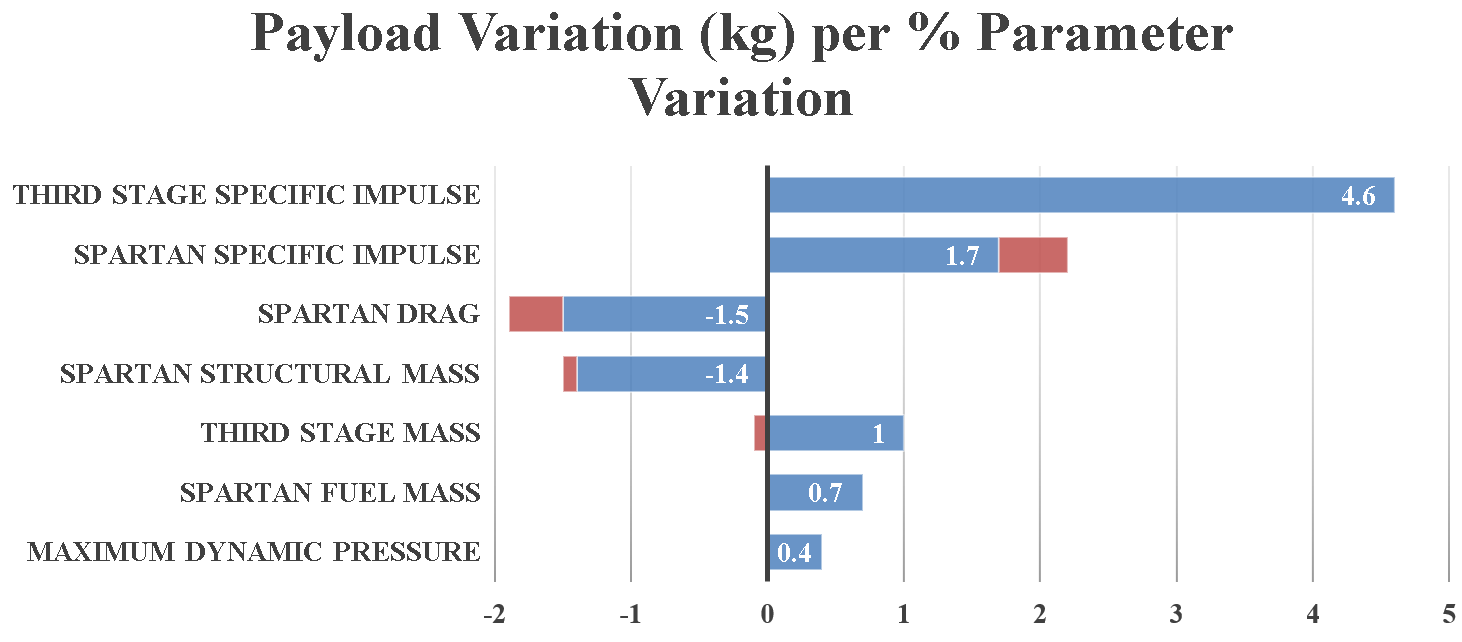
\includegraphics[width=0.8\linewidth]{figures/6_FlyBack/BarChart}
\caption{Sensitivity of design parameters. \textcolor{red}{include lines showing sensitivities without flyback}}
\label{fig:BarChart}
\end{figure}




\section{Sonic Boom Ground Effects}

The flight of a hypersonic vehicle has the potential to create significant overpressures on the ground due to sonic booms[CITEXX]. Even when the vehicle is flying at high altitudes, the overpressures on the ground may still be large enough to have detrimental effects on any populated areas being overflown. The overpressure from sonic booms can cause significant annoyance to the populace, or in more extreme cases, long term damage to building structures or peoples health. 
When the SPARTAN is launched to a sun synchronous orbit from the Equatorial Launch Australia launch site, it flies over a significant portion of Papua. Fortunately, Papua is sparsely populated, and the number of towns flown over by the SPARTAN will be low, however the effects on these population centres may still be significant. Although it is flying at high altitude, the SPARTAN is flying at hypersonic speeds, and creates significant sonic boom effects. In order to assess the impact of the SPARTAN's flight, the magnitude of the overpressure from its sonic booms must be calculated. 
\begin{figure}[ht]
	\centering
	\includegraphics[width=0.9\linewidth]{../LODESTAR_FINAL/Results/mode11/OverPressureStandard}
	\caption{}
	\label{fig:OverPressureStandard}
\end{figure}

The sonic boom overpressures are estimated using the 'first cut' estimation technique [CITEXX]. This estimation technique can approximate sonic boom overpressures moderately well, and is useful as a first approximation to the sonic boom overpressures generated by an aerospace vehicle. The overpressures generated by the SPARTAN are calculated over its trajectory, shown in Figure \ref{fig:OverPressureStandard}. It is found that overpressures of up to 375.3Pa occur during flight over land during the maximum payload-to-orbit trajectory of the SPARTAN. These overpressures have a low but significant probability of causing cosmetic damage to structures (~1.5\% for plaster and ~0.4\% for glass)[CITEXX-below]. In addition, overpressures of these magnitudes have been rated as unacceptably annoying to the majority populace being overflown, as shown in Figure \ref{fig:OverPressureResponse}. 
These overpressures indicate that overflight of populated areas may not be reasonable for the SPARTAN flying its maximum payload-to-orbit trajectory. 


%http://www.dtic.mil/dtic/tr/fulltext/u2/a028512.pdf





\section{Alternate Launch Locations}

A sun synchronous orbit may be attained in both northerly, and southerly directions. An alternate southerly launch is investigated for the rocket-scramjet-rocket launch system, in the case that flight over Papua is not possible. 


\begin{figure}[th]
\centering
\includegraphics[width=1\linewidth]{../LODESTAR_FINAL/Results/mode01/GroundTrackAlternate}
\caption{}
\label{fig:GroundTrackAlternate}
\end{figure}

\begin{table}
	\centering
\begin{tabular}{l c} 
	\hline \textbf{Trajectory Condition}
	& Alternate
	\\
	\hline \textbf{Payload to Orbit (kg)}
	& \PayloadToOrbitAlternate
	\\
	\textbf{Separation Alt, 1$\rightarrow$2 (km)}
	& \firstsecondSeparationAltAlternate
	\\
	\textbf{Separation v, 1$\rightarrow$2 (m/s)}
	& \firstsecondSeparationvAlternate
	\\
	\textbf{Separation $\gamma$, 1$\rightarrow$2 (m/s)}
	& \firstsecondSeparationgammaAlternate
	\\
	\textbf{Separation Alt, 2$\rightarrow$3 (km)}
	& \secondthirdSeparationAltAlternate
	\\
	\textbf{Separation $v$, 2$\rightarrow$3 (m/s)}
	& \secondthirdSeparationvAlternate
	\\
	\textbf{Separation $\gamma$, 2$\rightarrow$3 (deg)}
	& \secondthirdSeparationgammaAlternate
	\\
	\textbf{Separation $q$, 2$\rightarrow$3(kPa)}
	& \secondthirdSeparationqAlternate
	\\
	\textbf{2$^{nd}$ Stage L/D, 2$\rightarrow$3}
	& \secondthirdSeparationLDAlternate
	\\
	\textbf{2$^{nd}$ Stage Flight Time (s)}
	& \secondFlightTimeAlternate
	\\
	\textbf{3$^{rd}$ Stage $t$, $q >$ 5kpa (s)}
	& \thirdqOverFiveAlternate
	\\
	\textbf{3$^{rd}$ Stage max $\alpha$ (deg)}
	& \thirdmaxAoAAlternate
	\\
	\textbf{3$^{rd}$ Stage final v (m/s)}
	& \thirdcircvAlternate
	\\
	\textbf{3$^{rd}$ Stage final m (kg)}
	& \thirdcircmAlternate
	\\
	\hline 
\end{tabular} 
\end{table}

\section{Summary}
The fly-back trajectory of the SPARTAN hypersonic vehicle is investigated, from separation at 7.7$^\circ$S,145.0$^\circ$E to landing at 15.3$^\circ$S,144.9$^\circ$E, corresponding to a near 180$^\circ$ turn and a fly-back of 878km. The aerodynamics of the SPARTAN are calculated using CART3D, an inviscid CFD package, over the range of Mach numbers and angle of attack values of flight. The optimal trajectory of the SPARTAN is calculated, to fly-back to the initial launch position with minimum fuel. The optimal trajectory is calculated using the launch vehicle optimal control program LODESTAR. It is found that the SPARTAN is capable of returning to its initial launch position, using 166.0kg of fuel. The optimal trajectory terminates when SPARTAN reaches 200m altitude at a velocity of 119.8m/s. After this point, it is assumed that the SPARTAN lands on a traditional runway, at similar conditions to the space shuttle.  
This result indicates that the fly-back of a hypersonic launch vehicle from high velocity separation at a Mach number greater than nine, returning to its initial launch site using scramjet hypersonic airbreathing engines, is feasible. This fly-back to the the original launch site is a crucial component for low cost access-to-space using scramjets. 

The coefficient of drag of the SPARTAN and specific impulse of the scramjet engines were independently varied by $\pm10\%$ and the new optimal trajectories calculated to assess the robustness of the fly-back trajectory to uncertainties in vehicle aerodynamics and scramjet performance. It was found that a $\pm10\%$ variation in $C_D$ results in a +31.0\% or -34.9\% variation in fuel mass burned during fly-back, while a $\pm10\%$ variation in $I_{SP}$ results in a much smaller variation of -6.9\% or +13.8\%. These results indicate that the aerodynamics of a fly-back hypersonic accelerator are much more significant to the fly-back fuel usage than the performance of the scramjet engine. 

